

\chapter{Desenvolvemento da Unidade Didáctica}\label{chap:desenvolvemento}

\section{Fundamentación}
%• Fundamentación mediante a achega relevante e actualizada de documentos que versaren sobre a temática elixida e sustentada en achegas de investigación didáctica.

\section{Xustificación da unidade}
%• Xustificación da unidade atendendo á lexislación vixente (decretos, reais decretos de ensinanzas mínimas, e ordes), a outros aspectos psicopedagóxicos e didácticos que xustificaren a súa inclusión no currículo da etapa, e/ou o curso e a súa contextualización.

\section{Elementos da unidade didáctica}
%• Elementos da unidade didáctica claramente diferenciados e efinidos: expectativas de aprendizaxe (obxectivos e competencias básicas), contidos, temporalización, metodoloxía e recursos.

\subsection{Expectativas de aprendizaxe}
%Obxectivos e competencias básicas.

\subsection{Contribución ao logro das competencias clave}\label{sec-comp}
As competencias son as características que adquire unha persoa para que sexa capaz de realizar distintas tarefas. En \cite[p.~3]{aprsuperior} podemos ver que ``ademais de coñecementos e habilidades, a competencia implica a comprensión do que se fai e saber transferir''.

Na nosa proposta didáctica fomentamos a competencia de \textbf{Comunicación Lingüística (CCL)} obrigando ao alumnado a intervir na clase e a formular hipóteses sobre como pensa que se debería resolver un problema. Ao tratarse da materia de matemáticas, a \textbf{Competencia matemática e competencias básicas en ciencia e tecnoloxía (CMCCT)} trátanse durante toda a proposta. Ademais durante esta proposta empregamos frecuentemente o ordenador para diversas tarefas polo que a \textbf{Competencia Dixital (CD)} dos nosos alumnos é tratado. En menor medida intentamos que os alumnos adquiran competencias relativas a \textbf{Competencias sociais e cívicas (CSC)} e a \textbf{Aprender a aprender (CAA)} a través do traballo en grupo e da busca de información de algunha actividade.


\subsection{Contidos}
A secuencialización de \textbf{contidos} pretende responder a pregunta de que lle debemos ensinar aos alumnos. Intentaremos que durante o transcurso da implementación desta unidade didáctica, o alumnado adquira unha serie de conceptos, procedementos e actitudes. Durante esta proposta didáctica trataranse os seguintes contidos:

\begin{enumerate}[label=\bfseries Con\arabic*]
  \item\label{con1} Elementos básicos de xeometría. Punto, recta e plano.
  \item\label{con2} Posición relativa de rectas. Paralelismo e Perpendicularidade.
  \item\label{con3} Ángulos. Clasificación de ángulos en función da amplitude.
  \item\label{con4} Posición relativa de ángulos.
  \item\label{con5} Sistema sesaxesimal. Suma e resta de ángulos.
  \item\label{con6} Mediatriz e bisectriz.
  \item\label{con7} Polígono, concepto e partes. Clasificación polígonos por número de lados e ángulos.
  \item\label{con8} Triángulo. Clasificación triángulo por lados diferentes e ángulos.
  \item\label{con9} Suma dos lados dun triángulo.
  \item\label{con10} Puntos e rectas notables dun triángulo.
  \item\label{con11} Teorema de Pitágoras.
  \item\label{con12} Cuadrilátero. Clasificación cuadriláteros.
  \item\label{con13} Elementos dos polígonos regulares.
  \item\label{con14} Circunferencia, concepto e elementos.
  \item\label{con15} Círculo, concepto e elementos.
  \item\label{con16} Respecto polos compañeiros de traballo.
  \item\label{con16} Valoración da importancia da cooperación para realizar tarefas.
  \item\label{con17} Valoración da presenza das matemáticas en xeral e da xeometría en particular no día a día dos alumnos.
\end{enumerate}

\subsection{Temporalización}

\subsection{Metodoloxía}

Para a realización desta unidade didáctica empregaranse varias estratexias ou métodos de ensino-aprendizaxe que teñen en común que todos intentan, dentro do posible, que os alumnos e alumnas adquiran os coñecementos de forma significativa.

En paralelo as actividades levadas a cabo na clase, construíuse e actualizouse un blogue cos contidos dados na clase. Neste blogue ademais de expoñer de forma sintética unha explicación sobre o dado cada día, inclúense vídeos de profesores explicando estes contidos. Este modelo está moi relacionada coa \textbf{aula invertida} ou \textbf{flipped classroom}. En \cite[p. 1]{saez2014experiencia} vemos que este modelo consiste en ``prover aos alumnos de materiais audiovisuais, que lles resulten atractivos, e que lles faciliten os coñecementos teóricos que na ensinanza tradicional o profesor lles ofrecía na clase''. Na metodoloxía de aula invertida, o tempo de clase pasa a estar reservado para resolver dubidas, incidir máis nos contidos máis difíciles para o alumnado ou reforzar o aprendido a través do material audiovisual aportado.

Consideramos que esta metodoloxía levada a cabo na súa totalidade non é acertada no noso contexto pois por unha parte o seu éxito depende da responsabilidade dos alumnos e por outra parte aumentaría en gran medida o número de horas que o alumando ten que traballar na casa. Non obstante si que consideramos útiles usar vídeos para que os alumnos poidan repasar na casa algún concepto que non lles quedou claro de forma moito máis amena.

En algunhas das actividades empregamos a \textbf{gamificación} para motivar aos alumnos. En \cite{diaz2013potencial} vemos como a gamificación ``a través do uso de certos elementos presentes nos xogos que os xogadores incrementen o seu tempo nel así como a súa predisposición psicolóxica a seguir nel''. As características do alumnado actual na súa condición de residentes dixitais \cite{residentesdigitales} fai que necesiten maiores doses de motivación e predisposición para a aprendizaxe. Neste sentido, a conxugación adecuade destes elementos (gratificación, recoñecemento social, relación social, etc.) coa necesidade de motivación parece apuntar de forma case inexorable a dar unha importancia significativa á introdución do xogo na aprendizaxe \cite{gamificacion2}.

Durante esta proposta didáctica a gamificación empregase en maior ou menor medida durante as Actividades~3 (Sección~\ref{act3}) e na Actividade~13 (Sección~\ref{act13}). Nas dúas actividades detectouse como o nivel de implicación e de interese do alumnado aumentaba considerablemente con respecto o resto de actividades propostas.

A xeometría é un campo da matemática moi adecuado para a utilización de \textbf{materiais e recursos manipulables} para explicala. Segundo \cite{moreiro2010materiales},  o material manipulativo facilita os procesos de ensino-aprendizaxe dos alumnos, pois os alumnos experimentan situacións de aprendizaxe de forma manipulativa, que lles permite coñecer, comprender e interiorizar as nocións estudadas, por medio de sensacións. Durante a serie de actividades propostas empregouse material manipulativo durante as Actividades 8 (Sección~\ref{sec:sumang}), 15 (Sección~\ref{act15}) e 16 (Sección~\ref{act16}).

Outro dos recursos que se pode empregar na matemática e que pode colaborar en gran medida en sacala dentro do marco teórico no que parece estar metida é a \textbf{fotografía}. En \cite{gonzalez1989fotografia} descríbese unha experiencia levada a cabo neste sentido tamén no campo da xeometría. O autor resalta a importancia deste tipo de actividades nas que o fundamental non é a matemática pero que poñen ao alumnado en contacto con ela conseguindo sacala da aula e facerlle ver que existe na vida real.

Por último houbo certas actividades que, ben por non ser a contido a tratar apto para aplicar algunha da metodoloxía innovadora ou por non ocurrírsenos a forma de tratala desta forma, foron explicadas seguindo unha metodoloxía tradicional de \textbf{profesor transmisor de coñecemento}. Non obstante durante as explicacións destes contidos intentouse que o alumnado participase o máximo posible nas explicacións, volvéndose a clase máis que un monólogo do profesor, unha conversa entre este e o alumnado.

\subsection{Recursos}

\section{Medidas de atención a diversidade}
%• Atención á diversidade, coas estratexias e materiais para levala a cabo.


\section{Criterios e instrumentos de avaliación}
%• Criterios e instrumentos de avaliación e seguimento da unidade.

Os \textbf{criterios de avaliación} son as pautas que inciden na competencia do alumnado e permiten valorala de acordo cos retos co contexto actual~\cite[p. 134]{secdidac}. Hai que resaltar que a avaliación ten como misión non so poñer unha nota numérica senón sobre todo axudar a que o alumnado mellore as súas competencias indicándolle en que actividades obtivo un bo rendemento e en cales se debe incidir máis. Os criterios empregados nesta proposta son:

\begin{enumerate}[label=\bfseries Cri\arabic*]
  \item\label{cri1} Recoñecer elementos básicos de xeometría como punto, recta, ángulo. Clasificar estes elementos atendendo as súas propiedades e a súa posición relativa.
  \item\label{cri2} Calcular a suma e resta de ángulos expresados en unidades de sistema sesaxesimal.
  \item\label{cri3} Explicar as propiedades de mediatrices e bisectrices e saber trazar estes elementos.
  \item\label{cri4} Diferenciar elementos dos polígonos e clasificalos en función do número de lados e os seus ángulos.
  \item\label{cri5} Clasificar triángulos e cuadriláteros en función das súas propiedades.
  \item\label{cri6} Trazar os puntos e rectas notables dun triángulo e explicar as propiedades e a utilidade destes puntos.
  \item\label{cri7} Empregar o teorema de Pitágoras para a resolución de problemas xeométricos.
  \item\label{cri8} Explicar as propiedades das circunferencias e círculos e diferenciar os seus elementos.
  \item\label{cri9} Calcular a área e o perímetro de figuras planas a través da descomposición en polígonos. 
\end{enumerate}


\section{Secunciación das actividades}
%• Desenvolvemento completo das diferentes sesións de clase, incluídos os anexos co material completo e necesario para aplicar a unidade didáctica.

As actividades constitúen unidades de traballo dentro da nosa unidade didáctica. De seguido amósanse as actividades que se levaron a cabo durante esta proposta didáctica.

En paralelo as actividades que imos describir a continuación fomos actualizando un sitio web creado a tal propósito e que se pode visitar en \href{http://leirasmates.ga}{leirasmates.ga}. Neste blogue publicamos os contidos que se explicaron durante a clase e incorporamos fontes de información adicionais como poden ser vídeos de YouTube onde se explican os mesmos contidos de forma diferente ou artigos de outras páxinas web. No Apéndice~\ref{fich:blogue} pódense ver as entradas que se publicaron neste blogue.

\subsection{Act. 0: Fotografando a xeometría}\label{act0}

Propoñeremos esta actividade como unha tarefa que o alumnado deberá realizar na casa. Trátase dunha actividade introdutoria na que o alumnado deberá enviar por correo electrónico fotografías con elementos xeométrico que poidan atopar na súa contorna. Entregarémoslles unha ficha que se pode ver no  Apéndice~\ref{fich:act0} coas instrucións da actividade. Nesta ficha pedimos que busquen fotos onde saian dúas rectas paralelas, dúas rectas que non o sexan (secantes), un polígono de 3 lados (un triángulo), un polígono de 4 lados (un cuadrilátero), un polígono de 5 lados ou máis e dun círculo.

O obxectivo desta actividade é que as alumnas e alumnos tomen conciencia de que está rodeados de obxectos matemáticos e ao mesmo tempo obter material co que poder traballar tanto para a posición relativa de rectas como para a clasificación de polígonos.

\begin{figure}[h!]
  \centering
  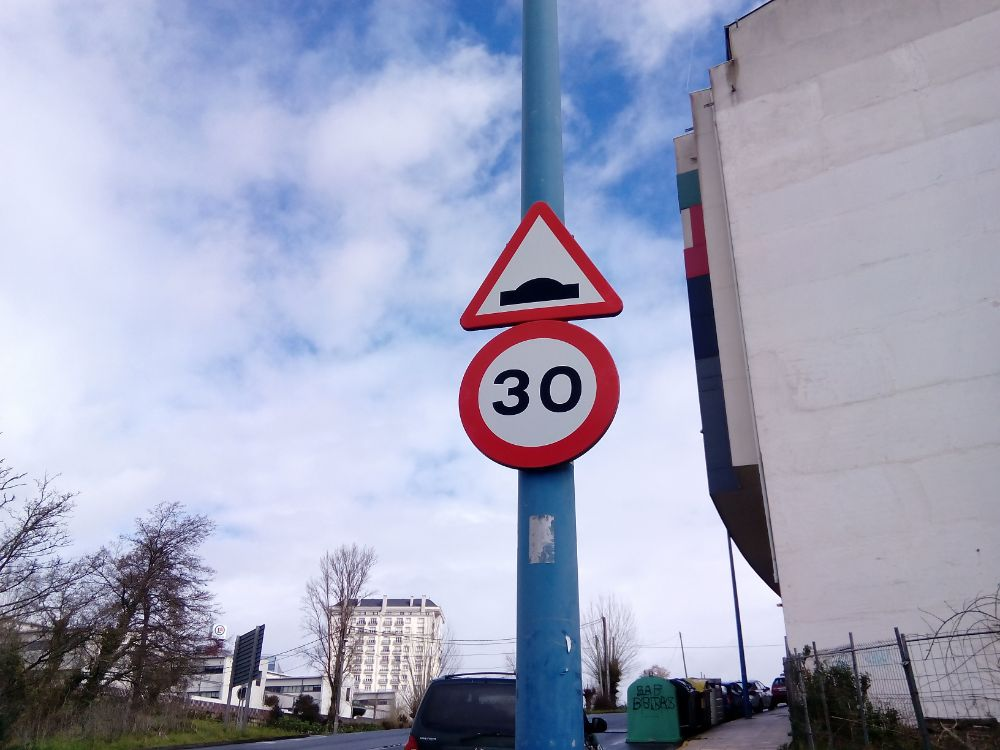
\includegraphics[height=4cm]{img/act0-1.jpg}
  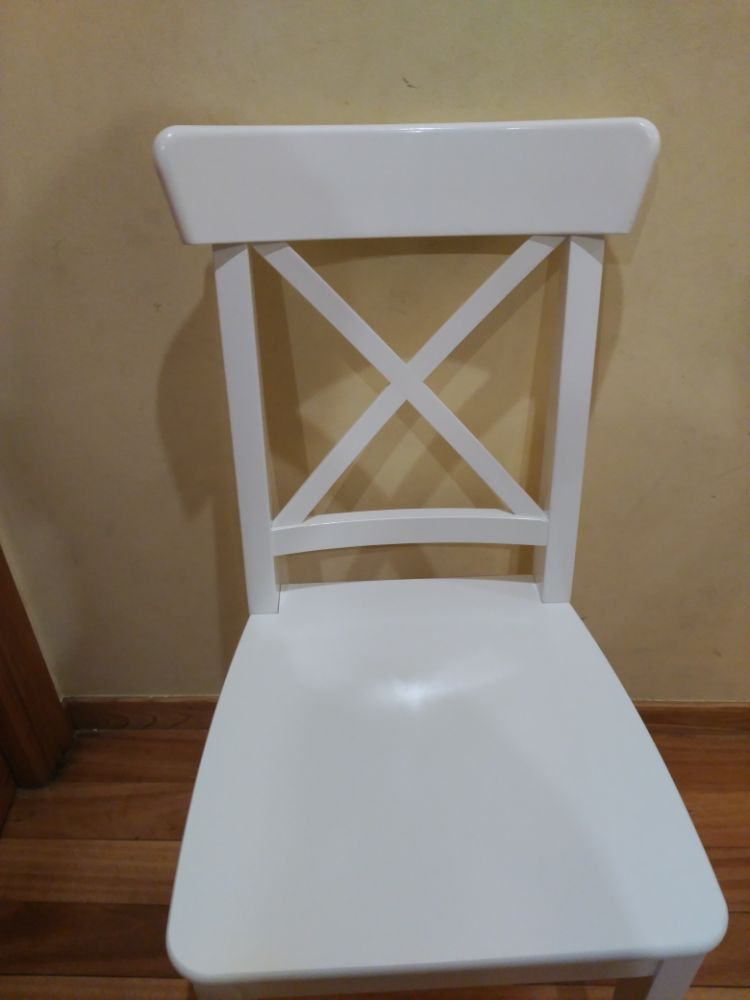
\includegraphics[height=4cm]{img/act0-2.jpg}
  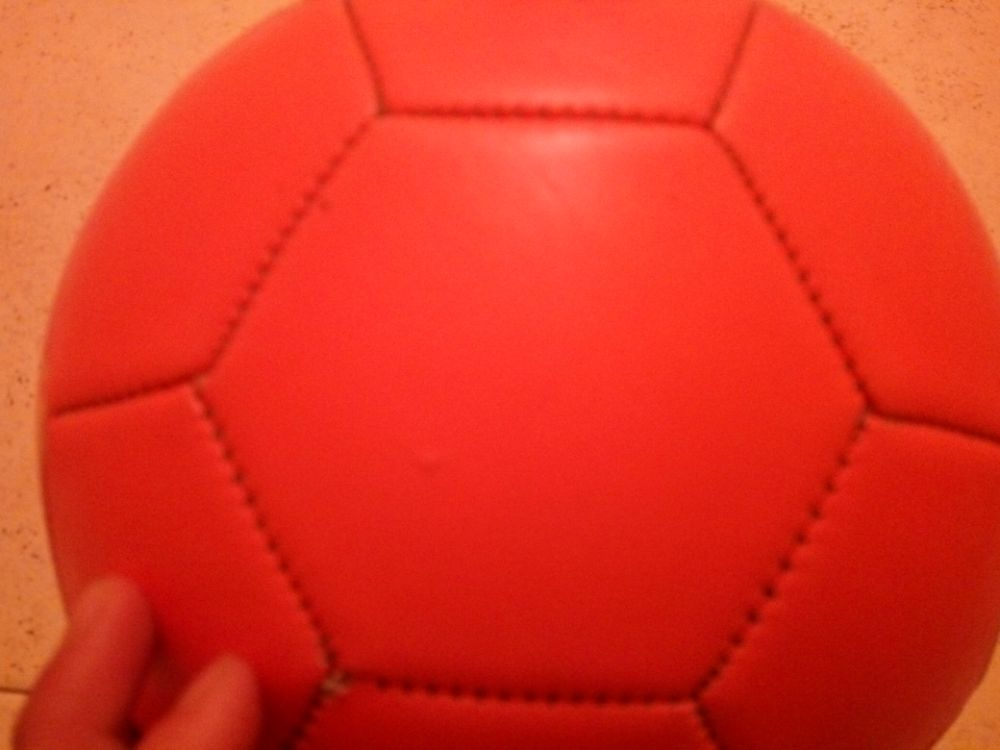
\includegraphics[height=4cm]{img/act0-3.jpg}
  \caption{Imaxes enviadas polos alumnos para a primeira actividade.}\label{fig:act0}
\end{figure}

Todas as fotos enviadas polo alumando serán subidas a web da materia. Na Figura~\ref{fig:act0} pódese ver algún exemplo do tipo de fotos que se buscan.

\subsection{Act. 1: Xeometría}
Como primeira activade do bloque de xeometría realizamos esta breve actividade introdutoria que pretende introducir ao alumnado no mundo da xeometría a par que se intenta habitualos nunha nova dinámica de clase na que se buscan a interacción docente-discente. Para introducilos no mundo da xeometría pedimos que definan coas súas palabras o que é a xeometría e a continuación mandarlles buscar por internet definicións de xeometría para que sexan lidas en voz alta. Para a realización desta actividade gastaremos sobre 10 minutos.

\subsection{Act.2: Puntos, liñas e posición relativa de liñas}\label{act2}
Durante esta actividade empezamos a explicar os elementos básicos de xeometría. Para facer isto comezamos preguntándolle aos alumnos e alumnas cal é para eles o elemento da xeometría máis simple que poden dicir. A raíz desta pregunta explicamos o concepto de punto. A raíz do punto explicamos que aliñando puntos obtemos unha recta. Explicase empregando un exemplo do programa Geogebra que a recta é infinita e que polo tanto non ten principio nin fin. A continuación expoñemos como se constrúe unha semirrecta, un segmento e detallamos a clasificación de rectas en función da súa posición relativa.

Para practicar a posición relativa das rectas realizamos unha actividade coas fotos de elementos xeométricos que enviaron na Actividade 0 (Sección~\ref{act0}). Durante esta actividade dividimos ha clase en grupos e cada grupo debe sinalar nas fotografías as rectas que sexan perpendiculares, secantes e paralelas. Para sinalar as rectas empregarase o programa de edición fotográfica, como pode ser GIMP.

\begin{figure}[h!]
  \centering
  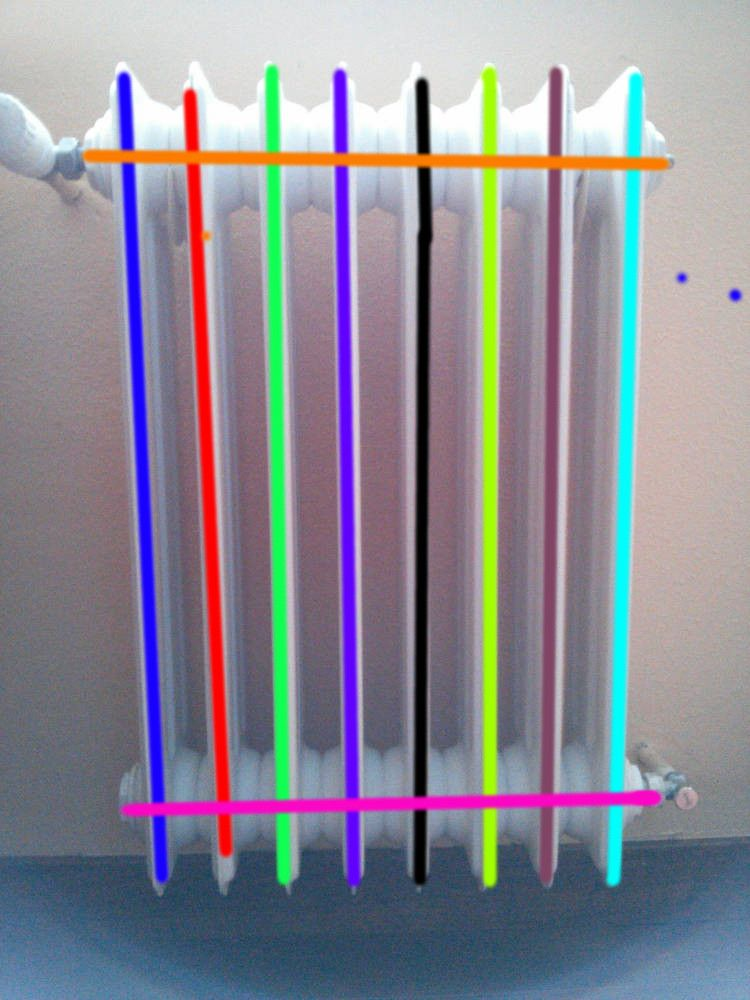
\includegraphics[height=4cm]{img/act1-img.jpg}
  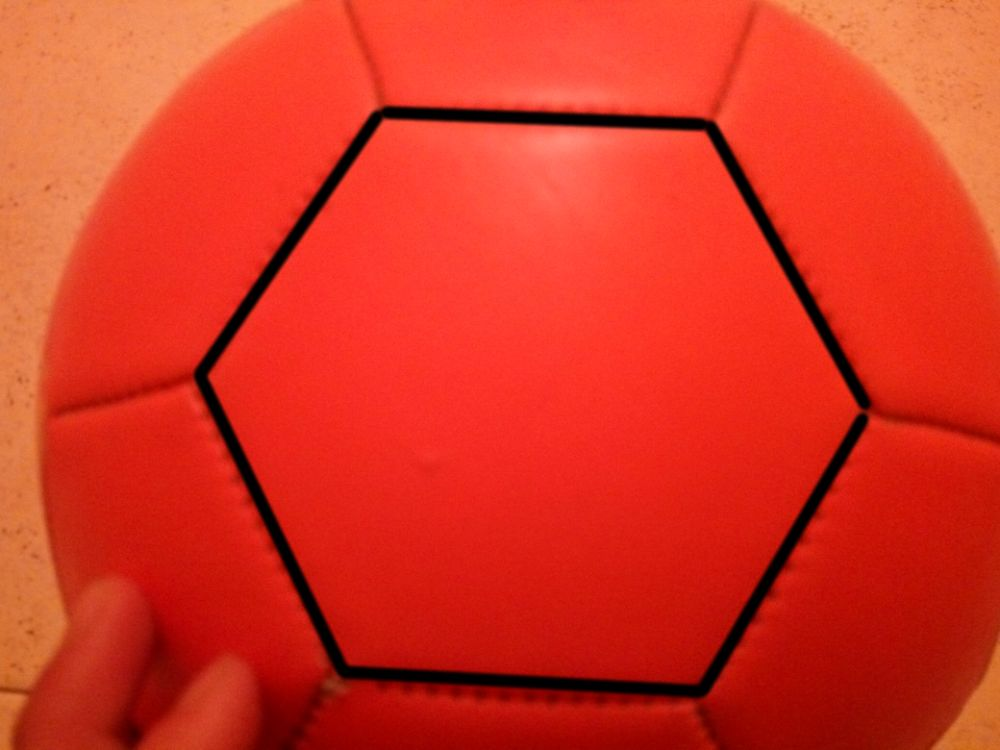
\includegraphics[height=4cm]{img/act1-img2.jpg}
  \caption{Marcado das imaxes con liñas paralelas, secantes e perpendiculares}\label{fig:act2}
\end{figure}

Despois de debuxar as rectas, os ficheiros son gardados e enviados por correo electrónico para ser proxectadas na clase. Cada grupo deberá explicar porque as rectas seleccionadoras teñen unha clasificación ou outra. Na Figura~\ref{fig:act2} pódense ver exemplos do que se pretende acadar. Dedicaremos a esta actividade aproximadamente 40 minutos.

\subsection{Act. 3: Ángulos e a súa clasificación}\label{act3}
Durante esta actividade explicaremos que é un ángulo así como a súa clasificación en función da súa amplitude e en función da súa posición relativa. Para practicar a clasificación de ángulos faremos un pequeno xogo onde as e os estudantes deberán por grupos clasificar diversos ángulos xerados aleatoriamente pola web \href{http://random.org}{Random.org}. Na Figura~\ref{fig:act5} pódese ver unha captura de pantalla dun ángulo xerado por esta web.

\begin{figure}[h!]
  \centering
  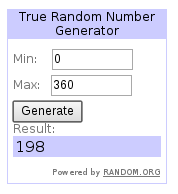
\includegraphics[height=5cm]{img/random.png}
  \caption{Captura de pantalla dun ángulo xerado por Random.org.}\label{fig:act5}
\end{figure}

\subsection{Act. 4: Sistema sexasesimal} %TODO
Explicamos o sistema sesaxesimal e como facer sumas e restas de grados expresados neste sistema. Baseamos a nosa explicación con unha comparación con algo que xa coñecen, a relación entre horas, minutos e segundos. Facemos varios exercicios propostos polo libro de texto sobre este tema.

\subsection{Act. 5: Mediatriz e bisectriz} %TODO
Explicamos os conceptos de mediatriz e de bisectriz e de como se trazan. Intentamos incidir nas propiedades que teñen a mediatriz e da bisectriz, e dicir, que os puntos destas dúas rectas equidistan dos extremos do segmento e dos lados do ángulo respectivamente. Estas propiedades serannos útiles máis tarde para explicar outros obxectos xeométricos como os puntos notables dos triángulos.

\subsection{Act. 6: Exame de xeometría básica}
Facemos un exame do explicado ata o momento que abrangue os conceptos de punto, rectas, planos, posición relativa de rectas, ángulos, clasificación de ángulos e posición relativa dos mesmos, sistema sesaxesimal, mediatrices e bisectrices. O exame que puxemos pódese ver no Apéndice~\ref{fich:ex1a}.

Intentando dar unha retroalimentación con respecto ao que o alumnado realizou neste exame o máis rápida posible corrixiremos os exercicios durante esa tarde e no día seguinte explicaremos todos os exercicios, os criterios de corrección e ensinámoslles ás alumnas e alumnos os exames corrixidos.

\subsection{Act. 7: Polígonos, triángulos e as súas clasificacións}\label{act7}
Expoñemos os conceptos de liña poligonal, de polígono e as clasificacións de polígonos en función dos seus ángulos e do número de lados. A continuación explicamos a clasificación dos triángulos en función dos seus ángulos e do número de lados iguais.

\begin{figure}[h!]
  \centering
  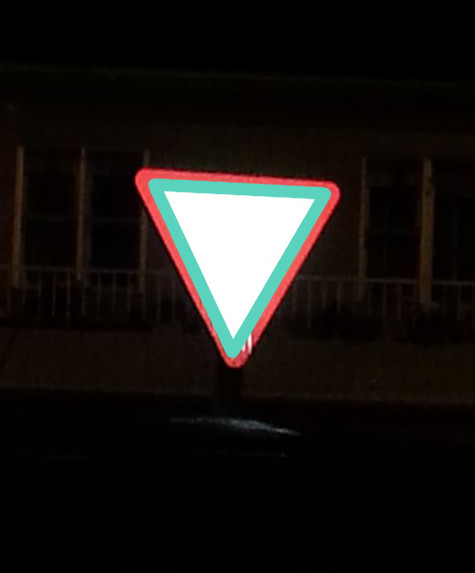
\includegraphics[height=5cm]{img/trian1.jpg}
  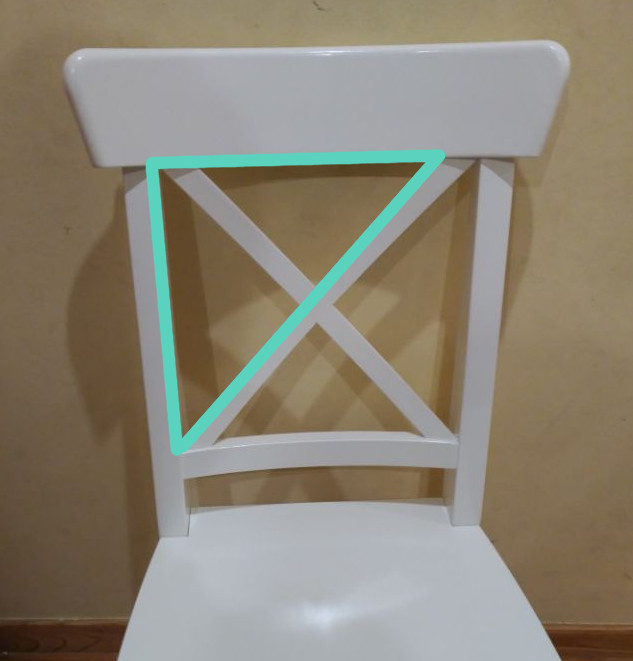
\includegraphics[height=5cm]{img/trian2.jpg}
  \caption{Exemplo de triángulo marcados sobre as fotografías}\label{fig:act7}
\end{figure}

Para practicar a clasificación dos triángulos realizamos un exercicio coas fotos que entregaron os alumnos durante a Actividade 0 (Sección~\ref{act0}). Para elo dividiremos a clase en grupos de 2 ou 3 persoas e cada grupo con un ordenador deberá buscar 4 triángulos diferentes nas fotos enviadas polos compañeiros. Da mesma forma que na segunda actividade, o alumnado deberá enviar as fotos editadas cos triángulos marcados ao ordenador do profesor no que se proxectarán. Cada grupo saíra e explicará a clasificación de cada un dos triángulos que marcou. Na Figura~\ref{fig:act7} pódense ver algúns exemplos das figuras que se pretenden acadar neste exercicio.

\subsection{Act. 8: Suma dos ángulos dun triángulo}\label{sec:sumang}
Nesta pequena actividade explicaremos e demostraremos de forma gráfica que a suma dos ángulos dun triángulo da sempre 180 grados. Para iso unha vez explicada esta propiedade na encerado, repartiremos triángulos feitos con goma-eva pero que, como se pode ver na Figura~\ref{fig:act11}, están partidos en tres fragmento de forma que se pode ver como poñendo os ángulos de forma consecutiva, obtense un ángulo llano.

\begin{figure}[h!]
  \centering
  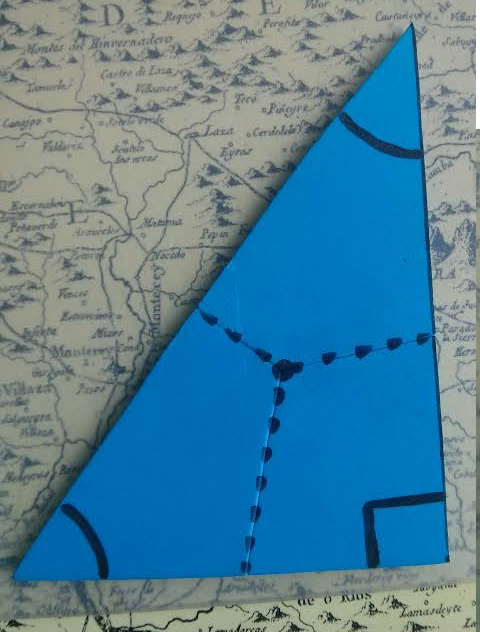
\includegraphics[height=5cm]{img/180grados-2.png}
  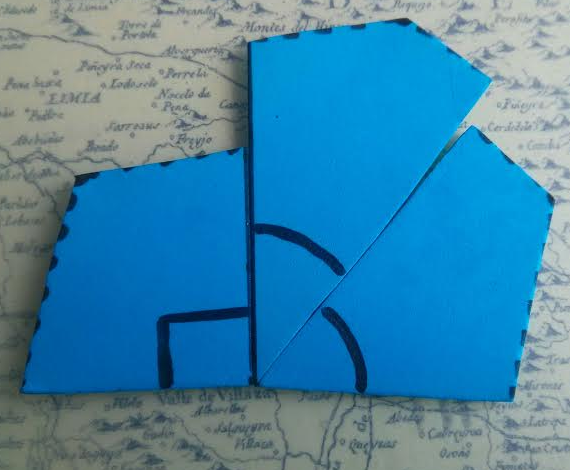
\includegraphics[height=5cm]{img/180grados-1.png}
  \caption{Figuras en goma-eva empregadas para ver a suma dos ángulos dun triángulo}\label{fig:act11}
\end{figure}

\subsection{Act. 9: Puntos e rectas notables do triángulo}\label{act9}
Explicamos os puntos e rectas notables recordamos primeiramente as definicións explicadas de mediatriz (como recta cuxos puntos equidistan dos extremos do segmento) e de bisectriz (como recta cuxos puntos equidistan dos lados do ángulo). Unha vez se repasaron estes conceptos, para explicar o circuncentro formulamos un problema no cal deberán buscar a posición ideal para colocar unha antena WiFi que abasteza ao instituto e a un hospital e centro comercial próximos. A formulación do problema acompoñámola coa imaxe que se pode ver na Figura~\ref{fig:act12-1}.

\begin{figure}[h!]
  \centering
  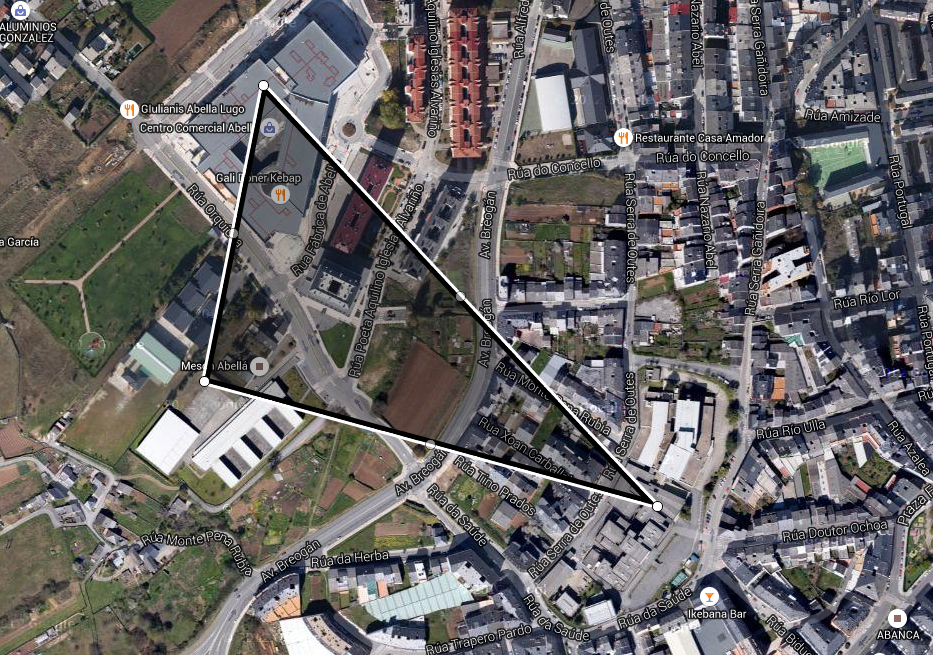
\includegraphics[height=5cm]{img/circuncentro.png}
  \caption{Imaxe empregada para explicar o circuncentro}\label{fig:act12-1}
\end{figure}

Pedimos que o alumnado formule como calcularían este punto e trázanse as solucións empregando o programa Geogebra. Explicamos porque as solucións propostas son ou non correctas e pedindo que expliquen porque a solución correcta consiste en trazar as mediatrices.

\begin{figure}[h!]
  \centering
  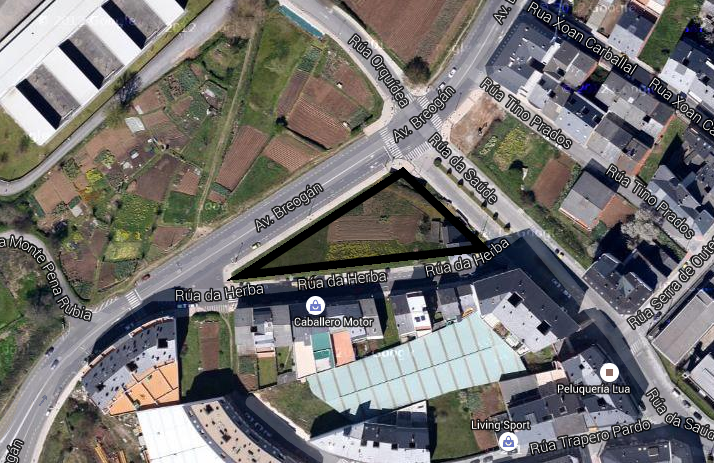
\includegraphics[height=5cm]{img/incentro.png}
  \caption{Imaxe empregada para explicar o incentro}\label{fig:act12-2}
\end{figure}

Para a explicación do dos demais puntos e rectas notables empregáronse métodos similares empregando a imaxe da Figura~\ref{fig:act12-2} para explicar o incentro e pedindo que dividan o triángulo en 6 partes de igual área no caso do baricentro.

\subsection{Act. 10: Teorema de Pitágoras}\label{act10}
Explicamos a denominación dos lados dun triángulo rectángulo e a relación entre a lonxitude destes. Relacionamos esta explicación coa area de cadrados con lados a hipotenusa e cada un dos catetos explicando que segundo o teorema cúmprese que a área do cadrado da hipotenusa é igual a suma das áreas dos cadrados dos dous catetos.

\begin{figure}[h!]
  \centering
  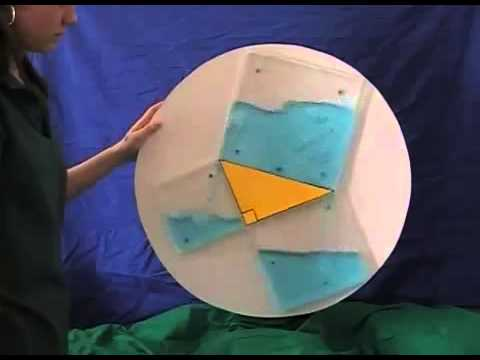
\includegraphics[height=7cm]{img/pitagoras.jpg}
  \caption{Captura dun dos vídeos proxectados con demostracións do Th. de Pitágoras}\label{fig:act10}
\end{figure}

Para reforzar o que explicamos na encerado proxectaremos varios fragmentos do documental \emph{Pitágoras: Mucha más que un teorema}\footnote{Este documental forma parte da serie Universo Matemático feito por RTVE que se pode ver completa en \href{http://www.rtve.es/television/la-aventura-del-saber/documentales/universo-matematico/}{rtve.es/television/la-aventura-del-saber/documentales/universo-matematico}.} relativos aos teorema. Ademais tamén se proxecta unha demostración feita con auga do teorema encontrada nun vídeo en YouTube\footnote{Pódese ver en \href{https://www.youtube.com/watch?v=1er3cHAWwIM}{youtube.com/watch?v=1er3cHAWwIM}.}. A captura da Figura~\ref{fig:act10} pertence a este último vídeo. Despois de ver estas demostracións, faremos exercicios propostos polo libro de texto.

\subsection{Act. 11: Clasificación cuadriláteros}\label{act11}
Explicamos a clasificación dos cuadriláteros e a continuación repetimos a mesma actividade que se realizou para practicar a clasificación dos triángulos.  Dividiremos a clase en grupos de 2 ou 3 persoas e cada grupo con un ordenador deberá buscar e marcar 4 cuadriláteros diferentes nas fotos enviadas durante a Actividade 0.
Os alumnos e alumnas enviaran as fotos modificadas ao ordenador do profesor para que estas sexan proxectadas e cada grupo lle poida explicar aos seus compañeiros a clasificación de cada un dos cuadriláteros que marcaron. Na Figura~\ref{fig:act11} pódese ver algún exemplo das figuras que pretendemos acadar.

\begin{figure}[h!]
  \centering
  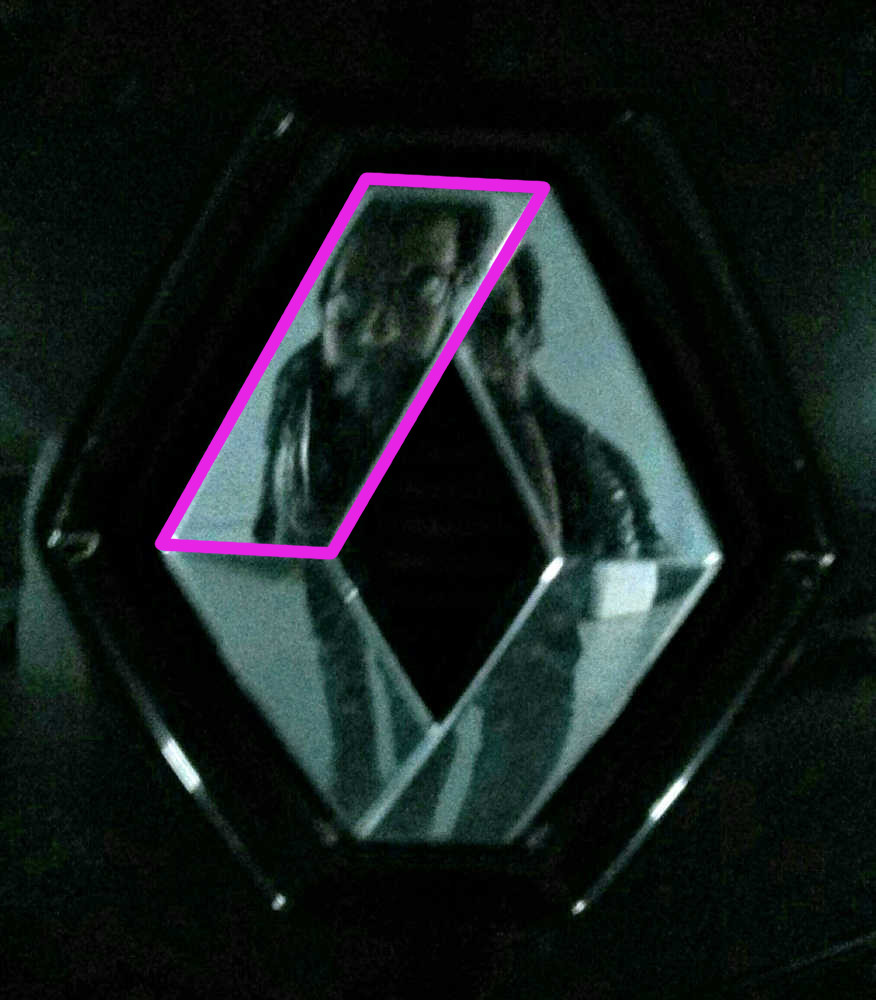
\includegraphics[height=5cm]{img/cuad1.jpg}
  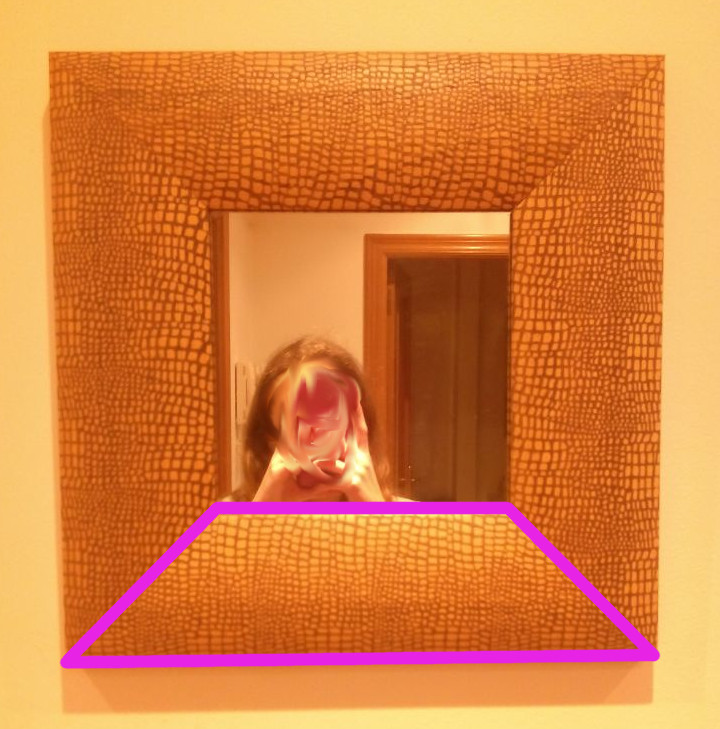
\includegraphics[height=5cm]{img/cuad2.jpg}
  \caption{Exemplo de cuadriláteros marcados sobre as fotografías}\label{fig:act11}
\end{figure}

\subsection{Act. 12: Elementos dos polígonos regulares. Circunferencia e círculo} %TODO
Durante esta actividade explicamos algún dos elementos dos polígonos regulares como o radio ou a apotema. Para explicar o concepto de circunferencia pedirémoslles ás alumnas e alumnos que formulen as súas propias definicións para ir corrixíndoas e terminar dando con unha correcta. Explicamos os elementos da circunferencia e por último o círculo e os seus elementos.

\subsection{Act. 13: Trivial de Polígonos}\label{act13}
Para practicar todos os conceptos traballados nas leccións anteriores trivial un trivial de 70 preguntas onde se repasan todos estes conceptos. Para facer isto empregamos a plataforma Socrative\footnote{Pódese acceder a ela en \href{http://www.socrative.com/}{socrative.com}.} que dispón dunha aplicativo móbil para a realización dos test así como a súa páxina web. Como se pode ver no Apéndice~\ref{fich:trivial}, as preguntas formuladas eran de varios tipos. Encontramos preguntas onde o alumnado debía seleccionar unha opción entre varias alternativas que lle eran dadas, preguntas onde debían dicir se un enunciado era correcto ou falso e preguntas onde eles mesmos debían escribir a resposta. Na Figura~\ref{fig:act13} pódese ver unha captura de unha posible pregunta que deberían responder as alumnas e alumnos.

\begin{figure}[h!]
  \centering
  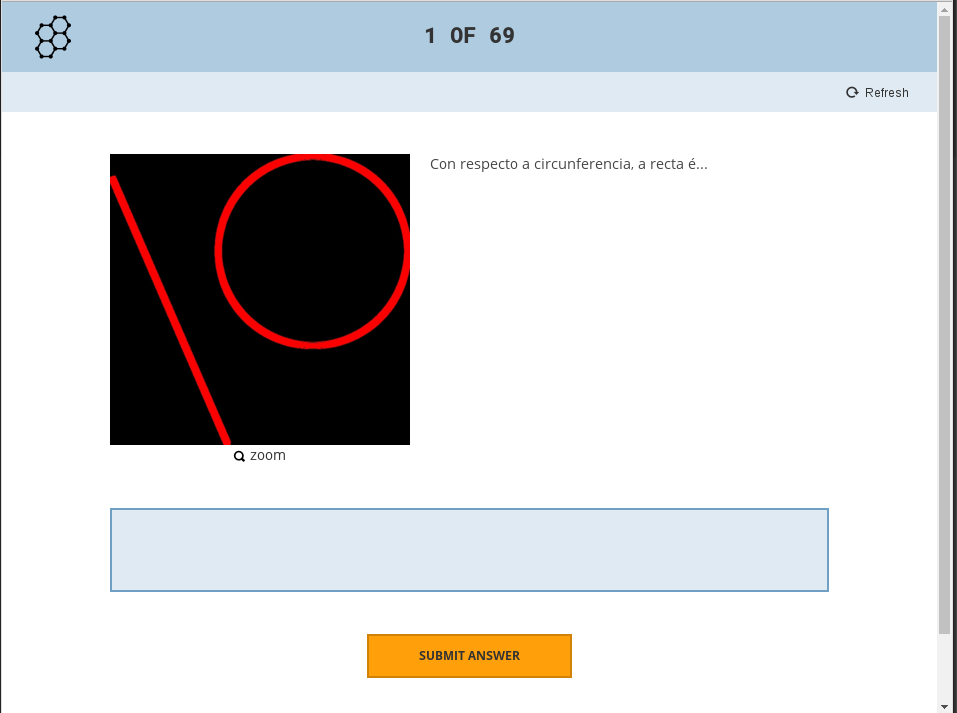
\includegraphics[width=0.8\textwidth]{img/socrative.png}
  \caption{Captura de pantalla dunha pregunta formulada na plataforma Socrative}\label{fig:act13}
\end{figure}

Para a realización do test dividiremos a clase en parellas e cada parella empregará un ordenador. Conectaranse á plataforma de Socrative e responderán a todas as preguntas durante a duración da clase. Durante a sesión seguinte a realización do trivial, analizaremos pregunta a pregunta cal é o resultado correcto e o porqué. Centrarémonos máis nos contidos que fallou a maior parte da clase.

\subsection{Act. 14: Exame polígonos}
Realizamos un exame dos contidos traballados anteriormente. O exame pode verse no Apéndice~\ref{fich:ex2}. Da mesma forma que fixemos no primeiro exame, corrixiremos os exames durante esa tarde para amosarllos ao día seguinte corrixidos e que reciban o \emph{feedback} o máis cedo posible.


\section{Valoración da aplicación da unidade}
%• Valoración da aplicación da unidade. Se por algunha circunstancia extrórdinaria non se puidese aplicar, a valoración referirase á idoneidade da unidade didáctica para o centro onde tiveron lugar as prácticas.